%% Master Thesis Template
%% Please update the specification through this link: https://daim.idi.ntnu.no/howto_thesis_submission.pdf

\documentclass[pdftex,10pt,b5paper,twoside]{book}
\usepackage[lmargin=25mm,rmargin=25mm,tmargin=27mm,bmargin=30mm]{geometry}

\usepackage{setspace}
\usepackage{graphicx}
\usepackage{amssymb}
\usepackage{mathrsfs}
\usepackage{amsthm}
\usepackage{amsmath}
\usepackage{color}
\usepackage{csquotes}
\usepackage{subcaption}
\usepackage[Lenny]{fncychap}
\usepackage[pdftex,bookmarks=true]{hyperref}
\usepackage[pdftex]{hyperref}
\hypersetup{
    colorlinks,%
    citecolor=black,%
    filecolor=black,%
    linkcolor=black,%
    urlcolor=black
}
\usepackage[font=small,labelfont=bf]{caption}
\usepackage{fancyhdr}
\usepackage[acronym]{glossaries}
\usepackage{times}
\usepackage[square,sort,comma,numbers]{natbib}
\usepackage{float}
\usepackage{multicol}

\usepackage{grfext}
\PrependGraphicsExtensions*{.pdf}

%\floatstyle{boxed} 
\restylefloat{figure}

\renewcommand*\contentsname{Table of Contents}

\pagestyle{fancy}
\fancyhf{}
\renewcommand{\chaptermark}[1]{\markboth{\chaptername\ \thechapter.\ #1}{}}
\renewcommand{\sectionmark}[1]{\markright{\thesection\ #1}}
\renewcommand{\headrulewidth}{0.1ex}
\renewcommand{\footrulewidth}{0.1ex}
\fancypagestyle{plain}{\fancyhf{}\fancyfoot[LE,RO]{\thepage}\renewcommand{\headrulewidth}{0ex}}


\begin{document}

\frontmatter

%% PART 1
%%The title page will be automatically generated and added by the DAIM system
\input{dedication.tex}		%% Optional

%% PART 2
\clearpage
\pagenumbering{roman}
\setcounter{page}{1}

\pagestyle{fancy}
\fancyhf{}
\renewcommand{\chaptermark}[1]{\markboth{\chaptername\ \thechapter.\ #1}{}}
\renewcommand{\sectionmark}[1]{\markright{\thesection\ #1}}
\renewcommand{\headrulewidth}{0.1ex}
\renewcommand{\footrulewidth}{0.1ex}
\fancyfoot[LE,RO]{\thepage}
\fancypagestyle{plain}{\fancyhf{}\fancyfoot[LE,RO]{\thepage}\renewcommand{\headrulewidth}{0ex}}

\section*{\Huge Summary}
\addcontentsline{toc}{chapter}{Summary}	
$\\[0.5cm]$

\noindent
Traditional \textit{Cellular Automata} (CA) transition tables grow quickly when the number of cell states or the size of the CA neighborhood increases.
For methods that search for good transition functions, such as genetic algorithms, the space of possible tables also grows rapidly with both parameters.
This paper investigates replacing the tables with \textit{Compositional Pattern Producing Networks} (CPPNs), a Neural Network-like encoding.
The search for good CPPN-based transition encodings is performed with the \textit{NeuroEvolution of Augmenting Topologies} (NEAT) genetic algorithm.

A software framework is implemented and the problems of 2D pattern morphogenesis and replication are investigated.
The results found are diverse, with some problems solved easily, some with moderate difficulty and some not at all.
The conclusion is that the idea shows promise, but further work is required to truly understand how the parts of the system interact and which configurations are suitable for which problems.

TODO update this

\clearpage
		%% Optional
\input{preface.tex}		%% Optional
\input{list.tex}			%% Generate TOC, list of tables, and list of figures automatically
%\section*{{\Huge Abbreviations}}
\addcontentsline{toc}{chapter}{Abbreviations}
$\\[0.5cm]$

\printglossary[title=Abbreviations]
	%% Optional

\cleardoublepage

\pagestyle{fancy}
\fancyhf{}
\renewcommand{\chaptermark}[1]{\markboth{\chaptername\ \thechapter.\ #1}{}}
\renewcommand{\sectionmark}[1]{\markright{\thesection\ #1}}
\renewcommand{\headrulewidth}{0.1ex}
\renewcommand{\footrulewidth}{0.1ex}
\fancyfoot[LE,RO]{\thepage}
\fancyhead[LE]{\leftmark}
\fancyhead[RO]{\rightmark}
\fancypagestyle{plain}{\fancyhf{}\fancyfoot[LE,RO]{\thepage}\renewcommand{\headrulewidth}{0ex}}

\mainmatter

%% PART 3 -- The Chapters
\chapter{Introduction}
\textit{Cellular Automata} (CA) were first conceptualized and introduced in the 1940's and 1950's.
Around the same time, the idea of the \textit{evolutionary algorithm} was also being developed independently.
Both of these concepts take inspiration from nature, and thus fall into the category of \textit{artificial life}.
One goal of this field of research is to create systems that are of complexity comparable to that of biological systems found in nature.

One way to try to achieve this goal is to combine these two distinct concepts: Cellular systems designed by evolution.
Many different kinds of tasks have been solved by cellular systems that have been created this way.
However, more complex tasks and more complex models means greater spaces of possible solutions that the evolutionary algorithm must search.
%This phenomenon is seen in many fields, and is often referred to as "the curse of dimensionality" (TODO citation).
For a traditional genetic algorithm it can be both time consuming and challenging to find good solutions.

One of the possible ways to remedy this problem is to replace the traditional table-based encoding of CA transition rules with a different encoding: an encoding that supports a more complex evolutionary algorithm.
This paper describes the investigation of using \textit{Compositional Pattern Producing Networks} (CPPNs) as the data structure for transition rules,
and the \textit{NeuroEvolution of Augmenting Topologies} (NEAT) genetic algorithm for evolving these CPPNs.

With CPPN-based transition functions there is not a linear relationship between the input-output size and the size of the encoding.
The algorithm starts with the smallest possible encoding and iteratively over time adds features to it and adjusts them until an optimal solution is found.
This \textit{complexification} mimics the process that biologists believe life on earth developed.

To test this new combination, which we call \textit{CA-NEAT},
a custom Python framework was built to run simulations in software.
The framework was tasked with solving various CA tasks of different difficulties, with different degrees of success.

TODO research question

TODO outline thesis
		%% Edit each chapter
\cleardoublepage
\chapter{Background \& Motivation}
\section{Complex and Biologically-Inspired Systems}
\epigraph
{
If you try and take a cat apart to see how it works, the first thing you have on your hands is a nonworking cat.
}
{Douglas N. Adams \\ \textit{The Salmon of Doubt} \cite{adams2002salmon}}

\begin{figure}
\centering
\includegraphics[width=.65\textwidth]{fig/complex_systems_sayama}
\caption[Complex systems taxonomy]{Complex systems taxonomy. Reproduced from \cite{sayama2015introduction} by Hiroki Sayama. TODO check that this figure is readable when printed B5}
\label{fig:complex_systems_taxonomy}
\end{figure}

\textit{Complex systems} is an umbrella category consisting of a variety of topics from a variety of domains, such as mathematics, computer science and biology.
Figure \ref{fig:complex_systems_taxonomy} shows one possible "taxonomy" of complex systems.
It is not immediately obvious why these topics should be grouped together.
The word \textit{complex} is related to \textit{complicated}, synonymous with \textit{difficult}, \textit{intricate} and \textit{perplexing} \cite{Thesaurus.com2017}.
In 1962, Herbert Simon proposed a definition as \textquote[\cite{simon1962architecture}]{made up of a large number of parts that interact in a non-simple way}.
Hiroki Sayama later elaborated this definition:
\blockquote[\cite{sayama2015introduction}]{
Complex systems are networks made of a number of components that interact with each other, typically in a nonlinear fashion.
Complex systems may arise and evolve through self-organization, such that they are neither completely regular nor completely random, permitting the development of emergent behavior at macroscopic scales.
}
By grouping these topics together,
it is possible to start seeing similarities across domains,
and find insights about one topic that may be applicable to other topics.

A common property of complex systems is \textit{emergence} over scale.
Sayama defines emergence as \textquote{a nontrivial relationship between the properties of a system at microscopic and macroscopic level}.
This means that a process which can be observed at the macroscopic level (e.g. the human body moving) can not be explained by studying the individual components that make up the system (looking at the cells that make up the body).
Instead, both the individual components and \textit{how they interact} must be understood.

The other common property of complex systems is \textit{self-organization} over time.
Sayama defines it as \textquote{a dynamical process by which a system spontaneously forms nontrivial macroscopic structures and/or behaviors over time}.
One example is magnetization of metals, where the initially random configuration of "spins" (the components of the larger system) orient themselves over time,
so that the magnetic vector of all the individual spins and that of the whole system become the same \cite{heylighen2001science}.

The behavior seen in complex systems can be characterized by these two properties.
Often the behavior is a combination of the two properties, rather than a clear instance of one or the other.

%Complex systems may have parameters that affect the outcome of the process they partake in.
%The term \textit{equifinality} is used to describe systems of different configurations that arrive at the same result TODO cite.

Many of the topics seen in Figure \ref{fig:complex_systems_taxonomy} are based on concepts found in nature.
These belong to the group of \textit{bio-inspired systems} and to the category of \textit{artificial life}.
Since the infancy of modern computing in the 1940s, computers have gradually gained the capability to perform many tasks.
Along the way, computer scientists and engineers have sometimes looked to nature for inspiration and goals to reach for.
Many times approaching problems from engineering, mathematical and logical perspectives have yielded good results.
But some times, the analytical approach leads to a dead end.
Some tasks that are trivial for a human to perform, can be practically impossible for a programmer to codify \cite{moravec1988mind}.
This is where the bio-inspired approach may help.
Since nature has been able to create biological "machines" that can solve these tasks, then perhaps borrowing nature's methods will allow computers to do the same.

\subsection{Morphogenetic Engineering}
The field of \textit{morphogenetic engineering} \cite{doursat2013review} studies the confluence between biological and artificial systems, and how to create new systems that straddle the the divide.
Doursat et. al. defined four categories of morphogenetic engineering that they classified existing techniques by:

\begin{description}
    \item[Category I: by Constructing] ~\\
        e.g. self-assembling robots
    \item[Category II: by Coalescing] ~\\
        e.g. swarm agents
    \item[Category III: by Developing] ~\\
        e.g. genetic algorithms
    \item[Category IV: by Generating] ~\\
        e.g. bio-inspired grammars
\end{description}

Within the third category we find many of the concepts that this thesis is concerned with, such as evo-devo and morphogenesis.

\section{Cellular Automata}
\textit{Cellular Automata} (CA) were first invented in the 1940s by John von Neumann and Stanislaw Ulam as mathematical models of computation \cite{von-neumann-1966}.
They were inspired by biological organisms,
and created a model that could emulate some of their interesting and useful properties,
such as multi-cellular development (e.g. embryogenesis), reproduction (clonal or sexual) and robustness (e.g. self-repair).

In the following decades, as modern computers emerged,
the concept of CA became the basis for the field of \textit{Cellular Computing} (CC).
As the performance of "conventional" computers kept increasing dramatically (as described by \textit{Moore's law})\cite{schaller1997moore},
CC never became the basis for the mainstream computers that we use today,
but CA and CC remained an area of research by mathematicians and computer scientists,
and as part of the larger field of artificial life.
More recently, as Moore's law has faltered and this rate of growth of performance has diminished,
some have started to look for new methods that can lead to renewed performance growth.
Parallel computing has helped a lot, but it has shown itself to be difficult in practice.
Some, such as Michael J. Flynn have speculated that CC might be the path forward \cite{flynn-1996} .
Matthew Cook proved that a CA of a certain configuration can be Turing complete \cite{cook-2004},
giving further credibility to this idea.

\subsection{CA Definition}
A CA consists of a grid of very simple units called cells.
A cell can be in one out of a finite set of states, and can change between states based on input to the cell.
As such the CA can be considered as a grid of identical Finite State Automatons.
Sipper \cite{sipper-1999} described the three core principles of CC, which also apply to CA in general:

\begin{description}
    \item[Simplicity]
        ~\\
        A cell is simple and can do very little by itself.
    \item[Vast Parallelism]
        ~\\
        The number of cells is very large, much more than the number of processors in a conventional parallel computer.
    \item[Locality]
        ~\\
        All interactions between cells take place on a purely local basis.
        No cell knows or controls the entire system.
\end{description}

The cells in a CA can "see" only their closest neighboring cells.
They use this limited information in conjunction with some set of rules to transition from one cell state to another.
Depending on the starting state of the whole system and the rules,
it is possible to observe interesting emergent or self-organizing behavior over time and space.
These interesting CA often find an \textit{attractor} \cite{gershenson-2004, wolfram1986theory}.
If a sequence of CA states repeat periodically it is called a \textit{cycle attractor}, and if the CA stabilizes into a permanent, fixed state is is called a \textit{point attractor}.
Figure \ref{fig:example_CA} shows an example of a CA that enters a cyclical attractor.
Binary CA, with only two possible cell states, are the most commonly seen and studied.
Greater numbers of cell states is possible, but the increase in degrees of freedom can lead to some problems.

\begin{figure}[h]
\centering
\includegraphics[height=0.4\textheight, width=\textwidth, keepaspectratio]{fig/result_figs/generate_mosaic/1}
\caption[Example CA]{An example binary 2D CA. At time step 5 the CA state is the same as that in time step 3, meaning the CA has entered a cyclical attractor with a period of 2 (oscillation).}
\label{fig:example_CA}
\end{figure}

%There are many properties of CA and of cellular computing that can be varied to produce different results \cite{sipper-1999}.
%In this paper we will define some further properties of CA as:
%\begin{itemize}
%    \item Structured as a 1D or 2D cartesian grid of cells.
%    \item Having uniform cells, sharing the same transition rules.
%    \item Having a finite discrete set of states that cells can have.
%    \item Synchronously changing states for all cells.
%\end{itemize}

%Examples that fit into this narrower definition include Von Neumann's cellular automaton \cite{von-neumann-1966}, Wolfram's elementary cellular automata (TODO cite) and Conway's Game of Life (TODO cite Conway).

%Figure \ref{fig:110} illustrates "elementarty CA 110", which has this property.
%This is an 1D CA, with successive states transitioning from the top to the bottom over time.
%Two different patterns stand out from the background.
%Over time they move towards each other and interact.
%This interaction is used in Cook's proof that CA 110 is Turing complete.
%
%\begin{figure}
%\centering
%\includegraphics[width=\columnwidth]{fig/110}
%\caption{Elementary CA 110
%(TODO cite \protect\url{https://commons.wikimedia.org/wiki/File:Ca110-interaction.png} properly)}
%\label{fig:110}
%\end{figure}

%Since the inception of CA by Ulam and Von Neumann in the 1940s \cite{von-neumann-1966},
%researchers have been interested in them for their biology-like properties and emergent behavior.
%Most implementations of CA have been formal mathematical works or simulations on conventional computers,
%but work has also been done with physical implementations using various substrates (TODO cite).
%
%In recent times the problem posed by the end of Moore's law and he difficulty of parallel computing with conventional architectures has caused cellular computing to become relevant again.
%Michael J. Flynn created Flynn's Taxonomy in 1966 \cite{flynn-1966}, describing different types of parallel systems.
%In 1996 he wrote a new article \cite{flynn-1996},
%outlining some of the difficulties that had hindered the expected parallel processing power that he and his peers had imagined back then.
%In this article he also described what he thought to be the road ahead, which is to represent problems in cellular form.

\subsection{Transition Rules}
\label{sec:transitions}
Langton \cite{langton-1990} formally defined finite CA as consisting of a finite set of cell states $\Sigma$ of size $K = |\Sigma|$,
a finite input alphabet $\alpha$, and a transition function $\Delta$.
Each cell has a $N$-sized neighborhood.
The number of possible neighborhood states can be expressed by equation \eqref{eq:kn}.

\begin{equation}\label{eq:kn}
    |\alpha| = |\Delta| = |\Sigma^N| = K^N
\end{equation}

The transition function for a CA must thus encode $|\alpha|$ different mappings of $N$ inputs to one of $K$ outputs.
The number of possible unique transition function behaviors is thus $K^{(K^N)}$.

\begin{figure}
\centering
\begin{subfigure}[t]{.175\columnwidth}
\centering
\includegraphics[width=\columnwidth]{fig/VonNeumann}
\caption{$N=5$ (Von Neumann)}
\label{fig:neighborhoods_vn}
\end{subfigure}\hfill%
\begin{subfigure}[t]{.175\columnwidth}
\centering
\includegraphics[width=\columnwidth]{fig/Moore}
\caption{$N=9$ (Moore)}
\end{subfigure}\hfill%
\begin{subfigure}[t]{.175\columnwidth}
\centering
\includegraphics[width=\columnwidth]{fig/LCR}
\caption{$N=3$}
\end{subfigure}\hfill%
\begin{subfigure}[t]{.40\columnwidth}
\centering
\includegraphics[width=\columnwidth]{fig/LLLCRRR}
\caption{$N=7$}
\end{subfigure}\hfill%

\caption[Some CA neighborhoods]{Some examples of common neighborhood shapes. The two common 2D shapes are named for John von Neumann and Edward F. Moore.
}
\label{fig:neighborhoods}
\end{figure}

\subsection{The $\lambda$ Parameter and the Edge of Chaos}
When Christopher Langton studied the elementary CA ($N=3, K=2$) \cite{langton-1990},
he created a metric to help determine if a rule is ordered, chaotic, or something in between, which he called $\lambda$.
It is defined by $K$, $N$ and the number of transitions that goes to the quiescent state, $n$.
\begin{equation}\label{eq:lambda}
    \lambda = \frac{K^N - n}{K^N}
\end{equation}

Langton found that low elementary CA $\lambda$ values resulted in ordered behavior, either settling into a static state or repeating periodically.
With high $\lambda$ values, the CA became chaotic, losing all useful information in the noise.
But at the critical border region between order and chaos, interesting behaviors and computation could occur \cite{langton-1990}.
This area has come to be called the \textit{edge of chaos}.

In the study Langton investigated the $\lambda$ of 1D binary CA, but the measure can be used on any CA.
The 2D binary transition function shown in Table \ref{tbl:example_CA} has 17 input combinations that lead to the quiescent ($0$) state ($n = 17$), and thus $\lambda \approx 0.47$.

\subsection{Finding Interesting Transition Functions}
\label{sec:finding_transitions}
\begin{table}
    \centering
    \caption[Example table-based transition rule]{
        An example table-based transition rule that exhibits the same behavior as seen in Figure \ref{fig:example_CA}.
        $N=5, K=2$ gives $|\alpha|=32$, the height of the table.
        The neighborhood shape is "Von Neumann" (Figure \ref{fig:neighborhoods_vn}).}
    \begin{tabular}{ccccc|c}
    North ($t_0$) & West ($t_0$) & Center ($t_0$) & East ($t_0$) & South ($t_0$) & Center ($t_1$) \\ \hline
    0      & 0      & 0      & 0      & 0      & 0        \\
    0      & 0      & 0      & 0      & 1      & 1        \\
    0      & 0      & 0      & 1      & 0      & 1        \\
    0      & 0      & 0      & 1      & 1      & 1        \\
    0      & 0      & 1      & 0      & 0      & 0        \\
    0      & 0      & 1      & 0      & 1      & 0        \\
    0      & 0      & 1      & 1      & 0      & 0        \\
    0      & 0      & 1      & 1      & 1      & 0        \\
    0      & 1      & 0      & 0      & 0      & 1        \\
    0      & 1      & 0      & 0      & 1      & 1        \\
    0      & 1      & 0      & 1      & 0      & 1        \\
    0      & 1      & 0      & 1      & 1      & 1        \\
    0      & 1      & 1      & 0      & 0      & 0        \\
    0      & 1      & 1      & 0      & 1      & 0        \\
    0      & 1      & 1      & 1      & 0      & 0        \\
    0      & 1      & 1      & 1      & 1      & 0        \\
    1      & 0      & 0      & 0      & 0      & 1        \\
    1      & 0      & 0      & 0      & 1      & 1        \\
    1      & 0      & 0      & 1      & 0      & 1        \\
    1      & 0      & 0      & 1      & 1      & 1        \\
    1      & 0      & 1      & 0      & 0      & 0        \\
    1      & 0      & 1      & 0      & 1      & 0        \\
    1      & 0      & 1      & 1      & 0      & 0        \\
    1      & 0      & 1      & 1      & 1      & 0        \\
    1      & 1      & 0      & 0      & 0      & 1        \\
    1      & 1      & 0      & 0      & 1      & 1        \\
    1      & 1      & 0      & 1      & 0      & 1        \\
    1      & 1      & 0      & 1      & 1      & 1        \\
    1      & 1      & 1      & 0      & 0      & 0        \\
    1      & 1      & 1      & 0      & 1      & 0        \\
    1      & 1      & 1      & 1      & 0      & 0        \\
    1      & 1      & 1      & 1      & 1      & 0        \\
    \end{tabular}
    \label{tbl:example_CA}
\end{table}

Traditionally $\Delta$ has been encoded as a complete mapping $\Delta: \Sigma^N \rightarrow \Sigma$, which can be implemented as a lookup table.
Table \ref{tbl:example_CA} shows an example of a table encoding for the CA in Figure \ref{fig:example_CA}.
This works very well for smaller cases such as the elementary CA.
But when working with non-trivial CA where both $K$ and $N$ can be relatively large numbers,
it becomes a problem both to store the mapping $\Delta$ in an efficient way,
and the space of possible $\Delta$ becomes too large to be explored by exhaustive enumeration.

Designing $\Delta$ with interesting behavior by hand is possible,
but it is time-consuming and impractical for problems of greater dimensions.
Using adaptive algorithms to explore the space of possible solutions is more feasible.
This is not guaranteed to produce good results though.
The use of table-based encodings put certain limitations on the search.
Using other encodings may enable new, more powerful search algorithms.
%This thesis concerns the investigation of a novel transition function encoding and associated search algorithm.

%\subsection{CA Problems}
%There are many kinds of problems that can be solved with CA.
%One class of problems is called \textit{morphology problems}.
%In these problems, the goal is for the CA to create some kind of complex structure.
%This can for example be \textit{morphogenesis}, where a simple structure is over time transformed into a more complex one,
%or it can be \textit{replication}, where some complex structure present initially must be copied.
%
%Another class of problems can be called \textit{information problems} (TODO is there a more appropriate term?).
%In this kind of problem the goal can be to compute some result based on the initial state, or to transmit information about state from one end to another.
%
%TODO citations

\section{Artificial Neural Networks}
\begin{figure}
\centering
\includegraphics[width=.5\columnwidth]{fig/Artificial_neural_network}
\caption[Example ANN]{
    An example layered ANN with three input neurons, one bias neuron, three hidden neurons and two output neurons.
    Each connection between neurons also has some weight that scales the value being passed (not shown).
}
\label{fig:ann}
\end{figure}

\textit{Artificial Neural Networks} (ANNs) \cite[Chapter 1]{bengio2015deep} have been used in many different applications related to artificial life and intelligence,
such as robotics or machine learning.
An ANN is a directed graph structure, with vertices (referred to as neurons) and edges (referred to as connections).
Input values are fed into the first layer of neurons and passed through the connections to the next layers.
All the connections to one neuron is added together and input to the neuron.
In each neuron some activation function transforms the input to a new value, and in each connection the value is scaled by some weight.
There can also be \textit{bias} neurons, outputting values that are constant, not determined by input.

This is inspired by neuroscience, with the brain consisting of neurons and synapse connections.
ANNs are useful because they consists of many discrete parts that can be individually or collectively tuned by some adaptive process,
and are easily expanded.
The \textit{universal approximation theorem} \cite{Hornik1989359} shows that relatively simple ANNs can approximate a wide variety of functions,
and the field of deep learning shows that a large complex structure with enough tuning can perform very complex tasks, such as image classification or natural language processing.
Figure \ref{fig:ann} shows an example ANN with three inputs and two outputs.
An example of a use case for this structure could be to control a robot with three sensors and two motors.

\subsection{Compositional Pattern Producing Networks}
\begin{figure}
\centering
\begin{subfigure}[b]{.25\columnwidth}
\centering
\includegraphics[height=5cm, keepaspectratio]{fig/2-cppn}
\caption{~}
\end{subfigure}\hfill%
\begin{subfigure}[b]{.65\columnwidth}
\centering
\includegraphics[height=5cm, keepaspectratio]{fig/cppn_pattern}
\caption{~}
\end{subfigure}

\caption[Example CPPN]{An example composition of the sigmoid, sinusoid and hyperbolic tangent functions.
The discrete coordinates of (b) are first normalized to $[-1.0, 1.0]$ and then mapped to various output values through the CPPN (a).
%The output pattern is visualized with different shades.
%The final neuron also has an activation function, but in this case it is the identity function, so no transformation is done.
}
\label{fig:cppn}
\end{figure}

A \textit{Compositional Pattern Producing Network} (CPPN) is an \textit{artificial development encoding} introduced by Kenneth O. Stanley in 2007 \cite{stanley-2007}.
CPPNs are structurally similar to ANNs, but differ in the use case.
Various techniques designed for ANN development and analysis may also be used for CPPNs.

Just like an ANN, a CPPN consists of a set of nodes with activation functions, weights and biases, as well as weighted connections between nodes.
Also like in an ANN, external values are input to the first layer, then undergo transformation by weights and activation functions before being outputted by the final layer.
This can be thought of as a composition of functions producing a pattern, hence the name.
An ANN is usually structured with neurons of the same activation functions,
arranged in layers,
whereas a CPPN has few such restrictions on topology and layer-wise heterogeneity.

%The difference between an ANN and a CPPN is subtle, and is primarily in the use case.
%With ANNs there is often a subset of the possible inputs that is considered "interesting" or "valid" inputs and produce interesting or valid outputs.
%With CPPNs the user is often interested in the entire mapping of all possible inputs to output and the pattern the outputs produce.
%Another difference is in the activation function of the neurons.
%In ANNs the neuron activation function is usually the same for all neurons,
%whereas in a CPPN the network consists of a variety of functions.
%The input to the network is transformed through this composition of functions.

Figure \ref{fig:cppn} shows an example CPPN and its output when mapped over a 2D Cartesian grid.
A CPPN is able to produce a pattern without multiple steps of development,
in contrast to e.g. a CA where local interactions and time is required.
CPPNs have been used both to produce patterns for the sake of the patterns, e.g. as evolutionary art \cite{stanley2006exploiting},
but also to create patterns which are used in a larger process,
such as machine learning \cite{d2008generative} and robot control \cite{risi2013confronting}.

%\subsubsection{CPPNs as CA Transition Functions}
%It is possible to use a CPPN as $\Delta$.
%The CPPN takes an $\alpha$ value as input and output a $\Sigma$ value.
%In terms of memory this CPPN $\Delta$ would not scale linearly with $K^N$.
%Because the space of possible CPPN structures is unconstrained,
%the solution space is unbounded, so some intelligent search heuristic is needed in order to find good $\Delta$ for a particular problem.


\section{Artificial Evolution and Development}
TODO rewrite

\textit{Artificial development} and \textit{artificial evolution} takes inspiration from biology in order to explore large and complex solution spaces for some given problem.

In a typical \textit{genetic algorithm} (GA) setup \cite{mitchell-2001},
relatively simple representations of solutions are encoded as \textit{genotypes} (also called \textit{genomes}).
Through some \textit{development process} a genotype may be transformed into a \textit{phenotype} which can be used to attempt to solve the problem at hand.
The performance of the phenotype at solving the problem is the \textit{fitness} of that individual genotype.

The fitnesses of a \textit{population} of different individuals are compared.
A selection process picks individuals from the population that get to reproduce.
This selection process is usually stochastic, with a bias towards picking the individuals with the highest fitness, but some chance of picking a less fit individual now and then.

Individuals that are selected for reproduction are paired up.
The genotypes of the pair are combined in some fashion to create a new genotype.
In addition to the combination, random mutations may also be applied in order to produce new features not present in either parent.
As new individuals are born, the older parent generation dies out, so that the entire population is replaced.
In some cases the very best individuals of the parent generation are cloned directly into the next generation,
ensuring that their well-performing genotype continues to be present until some better genotype comes along.
This is called \textit{elitism} \cite{vasconcelos2001improvements}.

Starting out with an arbitrary initial population and repeating this generational algorithm,
it is often possible to find novel genotypes that encode good solution to the problem at hand.
Like other algorithms that search a space of solutions,
there is a risk of getting stuck in a local maximum and never finding a global maximum,
an optimal solution to the problem at hand.
There are many kinds of parameters, such as mutation rate or selection function that can be tweaked to try to avoid this.

When a phenotype is developed into a genotype, it is either possible that the genotype encodes the entire phenotype explicitly,
or it is possible that the development process augments the information stored in the genotype to create a more complex phenotype.
This is called respectively \textit{direct} and \textit{indirect encoding} \cite{clune2011performance}.
Indirect encodings allows the evolutionary search to explore a space of genotypes that is smaller than the space of possible phenotypes.
This is the way development happens in nature, where simple genomes are developed into complex lifeforms \cite{clune2011performance}.

\subsection{NEAT}
\textit{NeuroEvolution of Augmenting Topologies} (NEAT) is a genetic algorithm variant introduced by Stanley and Miikkulainen in 2002 \cite{stanley-2002},
designed specifically to evolve ANNs.
When introducing CPPNs \cite{stanley-2007}, Stanley also introduced the CPPN-NEAT variation of the algorithm.

A NEAT genome consists of genes that encode nodes and connections between them.
Figure \ref{fig:neat} shows an example genotype to phenotype mapping.
NEAT starts with an initial population of very simple networks, typically with just the input and output nodes and connections between them.
Over generations, more nodes and vertices are added or disabled, activation functions are changed, and weights are adjusted.
The process of gradually expanding the genome is called \textit{complexification},
and reflects how life on earth is believed to have started with simple organisms and gradually evolved into more complex creatures \cite{darnell1986speculations,pross2005emergence}.

The genes that make up a NEAT genome are marked with an \textit{innovation number} so that they may be recognized as the same gene in different individuals.
As new features are added to the genomes, the individuals making up the population become gradually less similar.
The degree of similarity is measured through a measure called the \textit{compatibility distance}.
When the distance between individuals pass a certain threshold, they are segregated into separate species.
This process is called \textit{speciation}.
Pair selection for reproduction happens within species.
Typically the species that have the most fit individuals will produce more children,
while the less fit species will produce fewer (but not 0) children.

When a new species appears with a new feature,
the feature will not be tuned and likely affect the fitness of the individuals negatively.
NEAT protects new species for a certain amount of time,
allowing them time to adjust before being evaluated and, if performing poorly, being extincted to make more room for the more fit species.

\begin{figure}
\centering
\begin{subfigure}[t]{.5\columnwidth}
\centering
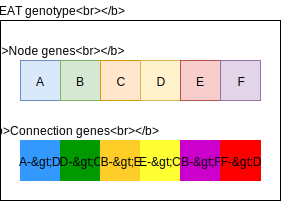
\includegraphics[height=5cm, keepaspectratio]{fig/NEAT_gt}
\caption{Genotype}
\end{subfigure}\hfill%
\begin{subfigure}[t]{.5\columnwidth}
\centering
\includegraphics[height=5cm, keepaspectratio]{fig/NEAT_pt}
\caption{Phenotype}
\end{subfigure}

\caption[Example NEAT genotype and phenotype]{
An example NEAT genotype and corresponding phenotype.
This example only shows the topology that the genotype encodes, leaving out the weights and activation functions.
}
\label{fig:neat}
\end{figure}

\begin{figure}
\centering
\includegraphics[width=\columnwidth, keepaspectratio]{fig/NEAT_mutation}
\caption[Example of NEAT mutation]{
    An illustrated example of NEAT mutation starting with a basic network of only two inputs and one output.
    Through the sequence neurons and connections are added until the network is equal to that in Figure \ref{fig:neat}.
    This example shows only mutation of genomes, leaving out the crossover operation which is also part of NEAT.
    }
\label{fig:neat_mutation}
\end{figure}


One notable use case of NEAT is called \textit{HyperNEAT} \cite{stanley2009hypercube}.
In this process, NEAT is used to evolve CPPNs whose output determine the topology of ANNs.
This is useful because it allows the ANN to scale easily, since the CPPN can just take more input and output more topology.
If the evolved CPPN has useful output at a small scale, it should also have a useful output at a large scale.

\subsection{Novelty Search}
\textit{Novelty search} is another genetic algorithm variant, introduced by Joel Lehmann and Kenneth O. Stanley in 2008 \cite{lehman-2008}.
It is good at \textit{deceptive} tasks, where local maximas in the fitness landscape do not lead to the global maximum, and thus "deceives" conventional algorithms.
Novelty search avoids this by eschewing the fitness measure entirely, and instead rewards \textit{innovation}, giving higher scores to genotypes that exhibit previously unseen behavior.
To find what behavior is new, an archive of seen behaviors is kept.
A \textit{distance metric} must be selected that is appropriate for the problem at hand.
For example, if the behavior of the phenotypes produces strings, an \textit{edit distance} measure such as the \textit{Levenshtein distance} can be used.
For each genotype the k nearest neighbors are found, and the average of these distances can be used as the \textit{novelty metric}.
If a new behavior is sufficiently novel, it is added to the archive.

TODO a bit more?


\cleardoublepage
\section{Related Work}
In \cite{wolper-2015}, Wolper and Abraham used evolution and CPPNs to find seed patterns for Conway's Game of Life \cite{berlekamp1982winning},
but not for finding transition rules.
They tried both normal CPPN-NEAT (objective search) and novelty search.
The results were varied, but the conclusion was in support of further research into using CPPNs for CA problems.

Many different kinds of CA encodings have been investigated previously.
With \textit{Conditionally matching rules} \cite{bidlo2013evolution, bidlo2015investigation, bidlo2015routine},
the table of transition rules is not a complete enumeration of all possible inputs,
but a sequence of conditions that, if all asserted, determine the next state of the cell.
In \textit{instruction-based development} \cite{bidlo2008instruction, bidlo2012evolution, nichele2016genotype,nichele2014evolutionary,nichele2016evolutionary},
the transition function encodes a set of instructions (a small program if you will) that transforms act on the input to produce the output.
With \textit{self-modifying cartesian genetic programming} \cite{harding2011self},
the transition function is a genetic program.
In \textit{variable length gene regulatory networks} \cite{trefzer2013advantages},
the genomes encode networks that mimic the network of cells found in nature.

Nichele and Tufte \cite{nichele2014evolutionary, nichele2016evolutionary, nichele2016genotype} has studied complexification during evolution,
both with table-based encodings and with instruction-based encodings.


\cleardoublepage
\chapter{Previous Work}
This thesis project is a continuation of a semester project done in the fall semester of 2016 at NTNU.
The project consisted of a period of development of the experiment framework, followed by a set of experiments.
A report was produced and TODO citation/link to report or paper
This chapter contains a brief summary of the results.
Implementation details of the framework is described in Section \ref{sec:implementation}.


\section{Scope}
The experiments in the previous project concerned the problems of two-dimensional morphogenesis and replication of a set of five "flag" patterns.
This is the same scope as that of \cite{nichele2014evolutionary}, which used an instruction-based encoding and also tested table-based encoding for comparison.
This allowed the results of \cite{nichele2014evolutionary} to act as a benchmark for testing the framework.

TODO make section about morhpogenesis and replication in background instead of explaining here?

\begin{figure*}[h]
\centering
\begin{subfigure}[b]{.20\textwidth}
\centering
\includegraphics[width=\textwidth]{fig/mosaic}
\caption{5x5 "Mosaic"}
\end{subfigure}%
\begin{subfigure}[b]{.20\textwidth}
\centering
\includegraphics[width=\textwidth]{fig/border}
\caption{6x6 "Border"}
\end{subfigure}%
\begin{subfigure}[b]{.20\textwidth}
\centering
\includegraphics[width=\textwidth]{fig/tricolor}
\caption{6x6 "Tricolor"}
\end{subfigure}%
\begin{subfigure}[b]{.20\textwidth}
\centering
\includegraphics[width=\textwidth]{fig/swiss}
\caption{5x5 "Swiss"}
\end{subfigure}%
\begin{subfigure}[b]{.20\textwidth}
\centering
\includegraphics[width=\textwidth]{fig/nordic}
\caption{7x7 "Nordic"}
\end{subfigure}%

\caption{Patterns being investigated.}
\label{fig:patterns}
\end{figure*}

The morphogenesis problem is defined as the development of a complex pattern from a simple "seed" pattern.
The biological analogy and inspiration is \textit{embryonic development},
with the seed pattern also referred to as \textit{zygote}.
Figure \ref{fig:seed} shows the seed patterns used in these experiments.

\begin{figure}[h]
\centering
\begin{subfigure}[b]{.30\columnwidth}
\centering
\includegraphics[width=\columnwidth]{fig/seed_5x5}
\caption{5x5}
\end{subfigure}%
\begin{subfigure}[b]{.30\columnwidth}
\centering
\includegraphics[width=\columnwidth]{fig/seed_6x6}
\caption{6x6}
\end{subfigure}%
\begin{subfigure}[b]{.30\columnwidth}
\centering
\includegraphics[width=\columnwidth]{fig/seed_7x7}
\caption{7x7}
\end{subfigure}%

\caption{Seed patterns for morphogenesis.}
\label{fig:seed}
\end{figure}

The replication problem start with one instance of some pattern in a larger grid,
and over time develop into a state where multiple copies of the pattern exists in the grid,
which may then replicate again.
The biological analogy of this is cell division and asexual (clonal) reproduction.
For the replication problem the seed pattern is thus one copy of the target pattern in a larger grid.
In these experiments the fitness evalutation function was configuired to require three perfect replicas for a perfect score.
Any additional replicas were not further rewarded.


\section{Results \& Discussion}
The results of the experiments were varied, with some problems being easily solved with CA-NEAT and other problems having few or no solutions found.
Table \ref{tbl:results} summarises the results in terms of success rate and generations of evolution.

\begin{table*}[h]
    \centering
    \caption[Summary of results]{
Summary of results.
The metrics shown are the success rate and the mean number of generations until a solution is found, with standard deviation also shown.
In the case of 100\% success rate, the number of generations column shows how many generations it took until the final solution was found.
In the case of less than 100\% success rate, the column shows how many generations were run until the experiment was stopped.
}
\begin{tabular}{lrrrr}
\hline
 Problem              &   Success rate \% &   Mean gens. &   $\sigma$ gens. &   Gens. until stop \\
\hline
Mosaic morphogenesis      &              100 &                1.2 &                 0.4 &                        2 \\
Border morphogenesis      &                1 &              270   &                 0   &                      509 \\
Tricolor morphogenesis    &              100 &               56.5 &               228.8 &                     2189 \\
Swiss morphogenesis       &               76 &              147.7 &               158.9 &                      600 \\
Mosaic replication        &              100 &                4.2 &                10.6 &                       99 \\
Swiss replication         &              100 &                7.7 &                 5   &                       20 \\
Tricolor replication      &               55 &               55.8 &                52.6 &                      200 \\
Nordic replication        &               0  &                  - &                   - &                      200 \\
\hline
\end{tabular}
\label{tbl:results}
\end{table*}

These results were compared with the results of \cite{nichele2014evolutionary}.
It was found that CA-NEAT was able to significanlty outperform instruction- and table-based encodings at some problems, while also performing much worse at other problems.
TODO more, summarize table

\begin{table}
    \centering
    \caption{TODO}
    \begin{tabular}{llll}
    \hline
    Problem                & Table-based & Instruction-based & CA-NEAT \\ \hline
    Mosaic morphogenesis   & 55\%        & 98\%              & 100\%   \\
    Swiss morphogenesis    & 23\%        & 100\%             & 76\%    \\
    Border morphogenesis   & 69\%        & 98\%              & 1\%     \\
    Tricolor morphogenesis & 19\%        & 46\%              & 100\%   \\
    Mosaic replication     & 85\%        & 100\%             & 100\%   \\
    Swiss replication      & 1\%         & 100\%             & 100\%   \\
    Tricolor replication   & 8\%         & 100\%             & 45\%    \\
    Nordic replication     & 0\%         & 100\%             & 0\%     \\ \hline
    \end{tabular}
\end{table}


Figures \ref{fig:tricolor_point_attractor} and \ref{fig:mosaic7} shows visualizations of two results found by evolution.
A larger selection of visualizations is available in the appendix of TODO.

\begin{figure}[h]
\centering
\includegraphics[height=0.4\textheight, width=\textwidth, keepaspectratio]{fig/result_figs/generate_tricolor/1}
\caption[A solution to the "Tricolor" morphogenesis]{A solution to the "Tricolor" morphogenesis that finds a point attractor equal to the target pattern.
Most solutions seen did not stabilize like this, but instead found a variety of cycles.}
\label{fig:tricolor_point_attractor}
\end{figure}

\begin{figure}[h]
\centering
\includegraphics[height=0.4\textheight, width=\textwidth, keepaspectratio]{fig/result_figs/replicate_mosaic/7}
\caption[A solution to the "Mosaic" replication]{A solution to the "Mosaic" replication that shows multiple stages of replication.
First the original replicates into two copies. Then each copy tries to replicate, but they interfere with each other and instead return to one copy each, but at a greater distance.
Then they each succeed in replicating, producing four copies total.}
\label{fig:mosaic7}
\end{figure}



\cleardoublepage
\chapter{Methodology}
\label{chap:methodology}

As this project is the continuation of work started in the previous semester,
some of the experiments in this project target the same problems as before,
with different methods in an attempt to get better results.
Other experiments target problems not previously attempted with CA-NEAT.

\section{CA-NEAT Implementation}
\label{sec:implementation}
TODO

\begin{figure}
\centering
\begin{multicols}{3}
\begin{enumerate}
    \item Sigmoid
    \item Hyperbolic tangent
    \item Sinusoid
    \item Gaussian
    \item Rectified linear unit
    \item Identity
    \item Clamped
    \item Inverse
    \item Logarithmic
    \item Exponential
    \item Absolute value
    \item Hat
    \item Square
    \item Cube
\end{enumerate}
\end{multicols}
\caption{Possible activation functions}
\label{fig:activations}
\end{figure}

\begin{figure}
\centering
\includegraphics[width=.5\columnwidth]{fig/single_layer_cppn}
\caption
[Example first-generation CPPN with 7 out of 10 possible connections.]
{Example first-generation CPPN with 7 out of 10 possible connections. $N=5$ input nodes corresponds to the "Von Neumann" neighbourhood shape, and $K=2$ output nodes correspond to a binary CA.}
\label{fig:single_layer_cppn}
\end{figure}

The nodes of the evolved CPPNs can have any of the activation functions listed in Figure \ref{fig:activations}.

\section{Novelty Search}
In order to extend CA-NEAT for novelty search, some phenotype value needs to be measured and compared in order to calculate novelty.
The enumerated "string" representation of the transition function was selected for this.
The \textit{Hamming distance} between different strings can then be calculated and used as a measure of novelty distance.

\section{Investigation of Genome Properties}
In order to gain a better understanding of the somewhat opaque GA process,
an experiment was designed with the goal of investigating the development of various properties of the population over time.

The "tricolor morphogenesis" was used as the basis for this experiment, since previous experiments with this problem showed it to be solvable, but not trivially simple for CA-NEAT.
The CA for this problem has $K=4$ cell states and the neighbourhood shape "Von Neumann" ($N=5$) was used.
An initial population of size $P=1000$ was created, with $N$ input nodes, $K$ output nodes and no initial hidden nodes.
This same population was then used as the initial population for five independent runs of $G=100$ generations, with different mechanisms of NEAT in use.
Table \ref{tbl:NEAT_incremental} shows which mechanisms are in use in which runs.

\begin{table}[h]
    \centering
    \caption{TODO}
    \begin{tabular}{c|ccccc}
    Run & Mutation & Crossover & Selection pressure & Speciation & Elitism \\ \hline
    A   & \checkmark        & ~         & ~                  & ~          & ~       \\
    B   & \checkmark        & \checkmark         & ~                  & ~          & ~       \\
    C   & \checkmark        & \checkmark         & \checkmark                  & ~          & ~       \\
    D   & \checkmark        & \checkmark         & \checkmark                  & \checkmark          & ~       \\
    E   & \checkmark        & \checkmark         & \checkmark                  & \checkmark          & \checkmark       \\
    \end{tabular}
    \label{tbl:NEAT_incremental}
\end{table}

Run A is a bit different, since it is not truly a GA run.
Instead the individuals that make up the population are mutated repeatedly, but crossover and elimination is not used.
Run B uses NEAT, however the selection is completely random, so there is no selection pressure.
Run C has selction pressure appropriate for the morphogenesis problem, but does not use the speciation mechanism of NEAT.
Run D is like C, but also uses the speciation mechanism.
And finally, run E uses all mechanisms of NEAT, including a pre-species elitism degree of $E=1$.

100 gens
    - only mutation
    - mutation + crossover, but fitness is constant
        -elitism=0
    - majority problem (do not stop scenario when f==1.0)
        -elitism=0?

investigate
    - lambda spread, mean, mode
    - genome size
    - change in enum-string
        - in terms of mean, median distance and bool(did change?)
    - amount of 'vestigial' nodes

\begin{figure}
\centering
\includegraphics[width=\columnwidth]{fig/mutation_behavior_change}
\caption{TODO}
\end{figure}

\begin{figure}
\centering
\includegraphics[width=\columnwidth]{fig/vestigial_nodes}
\caption{TODO}
\end{figure}

\begin{figure}
\centering
\includegraphics[width=\columnwidth]{fig/unique_behaviors}
\caption{TODO}
\end{figure}

\section{2D Morphogenesis With Coordinate Inputs}
TODO

\section{Majority Problem}
The majority problem is a problem for binary CA.
An arbitrary initial configuration should have one "color" be more common than the other.
The CA must figure out which color this is and end up in a point attractor state where all the cells are this color.
Depending on the initial configuration this can be very difficult.
Even if the majority of the configuration is black, there might be a sub-region that is majority white.
The lack of global overview means that the CA needs to send "signals" around and "negotiate" a consensus.

\section{Synchronization Problem}
Another problem for binary CA is called the \textit{synchronization problem}.
From some arbitrary initial configuration,
the CA should find its way to a two-step cyclic attractor where all cells share the same state in one timestep,
then all share the other state in the next timestep.
It is thus simillar to the majority problem in the way information must be transmitted across the CA in order to coordinate the cells,
but instead of having to "count" cells and landing in a specific point attractor, it finds a cyclic attractor without concern for which of the two states it visits first.

The fitness evaluation function for this experiment is based on the one described in \cite{das1995evolving}, but with some modifications.
$K=100$ random initial CA configurations are generated from a TODO distribution.
Each candidate solution is first tested on $I=25$ initial configurations.
If none of the $I$ configurations results in the desired behavior, a fitness of $0.0$ is reported.
If any of the configurations does result in the desired behavior, the candidate is tested on all $K$ configurations.
The fitness reported is then the ratio of configurations that show the correct behavior.


\section{Firing Squad Synchronization Problem}
TODO

\section{Novelty Search}
In order to extend CA-NEAT for novelty search, some phenotype value needs to be measured and compared in order to calculate novelty.
The enumerated "string" representation of the transition function was selected for this.
The \textit{Hamming distance} between different strings can then be calculated and used as a measure of novelty distance.


\cleardoublepage
\chapter{Discussion \& Future Work}
The individual experiments are discussed in their sections in Chapter \ref{chap:experiments}.
This chapter discusses the overarching themes, what went well and not so well, and the possibilities for future work.

\section{Morphology Problems}
Morphology of all the patterns in Figure \ref{fig:patterns} has been achieved,
either using only neighborhood information or using neighborhood information in conjunction with coordinate information.
In comparison with table-based and instruction-based evolution, CA-NEAT did better than either in most cases.

Replication was only tested with neighborhood information,
and the results were in general better than the corresponding results with table-based evolution,
though not as good as the results of instruction-based evolution.
With positive results from the morphogenesis with coordinate information,
it seems likely that the replication performance can also be improved by adding information to the environment.
For example, the environment could be augmented with "anchor points" in cells at intervals, giving the CA something to "latch on to" when producing duplicates.

\section{Computational Problems}
TODO

\section{The Role of CA-NEAT Mechanisms and Parameters}
TODO

\section{Novelty Search}
The choice of the enumerated mapping string to measure the innovation distance between phenotypes in novelty search has some disadvantages.
It "reintroduces" the restrictions of table-based transition functions to CA-NEAT.
It can't handle other types of input (e.g. like in Section \ref{sec:morphXY}),
and as the size of the neighbourhood or the number of cell states increases, so does the computational complexity of creating the strings and comparing them.

This does not mean CA-NEAT and novelty search are incompatible.
Other properties of the CA-NEAT transition function could be used to measure innovation distance.
These properties could be task-specific.
For example, in a morphogenesis task where finding a point attractor is required, the final (stable) state of the CA could be used as a vector,
and distance calculated appropriately.

When implementing CA-NEAT, the choice of database for persisting results was a relational (SQL) database.
When CA-NEAT was extended to novelty search, this meant that the innovation archive was also implemented as relational table.
As the innovation archive grew larger during experiments, it became obvious that this had a large detrimental effect on the performance of the algorithm, both in terms of time spent calculating and in terms of memory used during calculations.
The whole innovation archive was loaded into memory,
and the Hamming distances were calculated between the whole generation of individuals and the whole of the archive.
If implementing novelty search from scratch, a more suitable database structure could be used instead.
Inspiration could be taken from the techniques used in embedding spaces in machine learning applications.

Another possible option is to use the innovation archive population as a diverse initial population for normal NEAT.
It is possible some of the genotypes in the archive are close to, but not quite optimal, and that some generation of objective search evolution could lead to optimal results.
It would probably be neccessary to sample the archive though, as it may be much larger than the size of a population in normal NEAT.

\cleardoublepage
\chapter{Conclusion}
TODO

Novelty search is not to be written off, but problem-specific novelty metrics are needed to succeed.

\cleardoublepage

%% PART 4
\input{references.tex}	%% Edit your references in "mylib.bib"
%\section*{\begin{center}{\Huge Appendix}\end{center}}
%\addcontentsline{toc}{chapter}{Appendix}
%$\\[0.5cm]$

\appendix
%\renewcommand{\thesubsection}{\Alph{subsection}}

\chapter{CA-NEAT Parameters}
\label{app:parameters}
CA-NEAT has a large number of parameters that affect the outcome of the experiments.
This appendix lists some notable ones that would be needed to reproduce the results in this thesis consistently.

\begin{lstlisting}[language=Python, caption={
Parameters that define the initial population.
Notably, for each generated individual,
the ratio of connectivity is determined individually to be a value between $0.5$ and $1.0$.
}]
    initial_hidden_nodes = 0
    initial_connection = 'partial'
    connection_fraction = lambda *args: 0.5 * (1 + random.random())
\end{lstlisting}

\begin{lstlisting}[language=Python, caption={
Parameters that have to do with selection and speciation
}]
    survival_threshold = 0.2
    stagnation_limit = 15
    compatibility_threshold = 3.0
    excess_coefficient = 1.0
    disjoint_coefficient = 1.0
    weight_coefficient = 0.5
\end{lstlisting}

\begin{minipage}{\linewidth}
\begin{lstlisting}[language=Python, caption={
Parameters that have to do with mutation
}]
    max_weight = 30
    min_weight = -30
    weight_stdev = 1.0
    prob_add_conn = 0.5
    prob_add_node = 0.5
    prob_delete_conn = 0.25
    prob_delete_node = 0.25
    prob_mutate_bias = 0.8
    bias_mutation_power = 0.5
    prob_mutate_response = 0.8
    response_mutation_power = 0.5
    prob_mutate_weight = 0.8
    prob_replace_weight = 0.1
    weight_mutation_power = 0.5
    prob_mutate_activation = 0.002
    prob_toggle_link = 0.01
\end{lstlisting}
\end{minipage}

		%% Optional

\end{document}
